\documentclass[pageno]{jpaper}

%replace XXX with the submission number you are given from the ASPLOS submission site.
\newcommand{\asplossubmissionnumber}{289}

\usepackage[normalem]{ulem}
\usepackage{graphicx}
\usepackage{amsmath}
\usepackage{xcolor}
\usepackage{fancyhdr}
\usepackage{hyperref}
\usepackage{bbm}
\usepackage{times}
\usepackage{soul}
\usepackage[utf8]{inputenc}
\usepackage{latexsym}
\usepackage{amsmath}
\usepackage{graphicx}
\usepackage{caption}
\usepackage{subcaption}
\usepackage{amssymb}


%\usepackage[colorinlistoftodos]{todonotes}
\usepackage{algorithm}
\usepackage{algpseudocode}
%\graphicspath{ {images/} }
%\usepackage[square,sort,comma,numbers]{natbib}

\usepackage{float}
\floatstyle{plaintop}
\restylefloat{table}

\usepackage{graphicx,epstopdf}
\epstopdfsetup{update}
\DeclareGraphicsExtensions{.ps}
\epstopdfDeclareGraphicsRule{.ps}{pdf}{.pdf}{ps2pdf -dEPSCrop -dNOSAFER #1 \OutputFile}


\usepackage{stackengine}
\def\delequal{\mathrel{\ensurestackMath{\stackon[1pt]{=}{\scriptstyle\Delta}}}}

\begin{document}

\title{SECS: Efficient Deep Stream Processing via Class Skew Dichotomy}
\author{}
\date{}
\maketitle

\thispagestyle{empty}

\begin{abstract}
Despite accelerating CNNs receives an increasing research focus, the save in resource consumption always comes with a decrease in accuracy. To both increase accuracy and decrease resource consumption, we explore an environment information, called \textit{class skew}, which is easily available and exists widely in day-to-day life. Since the class skew may switch as time goes, we bring up \textit{probability layer} to utilize class skew without any overhead during the runtime. Further, we observe \textit{class skew dichotomy} that some class skew may appear frequently in the future, called \textit{hot class skew}, and others will never appear again, called \textit{cold class skew}. Inspired by techniques from source code optimization, two modes, i.e., interpretation and compilation, are proposed. The interpretation mode pursues efficient adaption during runtime for cold class skew and the compilation mode aggressively optimize on hot ones for more efficient deployment in the future. Aggressive optimization is processed by class-specific pruning and provides extra benefit. Finally, we design a systematic framework, SECS, to dynamically detect class skew, processing interpretation and compilation, as well as select the most accurate architectures under the runtime resource budget. Evaluations on recognizing faces in TV shows and movies show that SECS can realize end-to-end classification speedups of xxx/xxx (on GPU/CPU) relative to a state-of-the-art convolutional neural network, at competitive accuracy.
\end{abstract}




\section{Introduction} \label{Introduction}
% Need six paragraphs

Modern convolutional neural networks (CNNs) has made unprecedented advance in visual recognition tasks. In 2012, AlexNet \cite{krizhevsky2012imagenet} achieved a top-5 error of 17\% on ImageNet \cite{deng2009imagenet}, while previous method could only achieve a top-5 error of 25.7\%. Since then, CNNs have become the dominant method and main research direction in image recognition. In 2015, ResNet \cite{he2016deep} achieved a top-5 error of 3.57\%, supressing the human-level classification error rate on ImageNet reported as 5.1\% \cite{russakovsky2015imagenet}. The success of CNNs on visual recognition tasks has fueled the desire to deploy these networks on various kind of mobile platforms and has an increasingly important role in daily life, e.g., in robotics, self-driving cars, and on cell phones. These mobile platforms usually are memory-constrained and energy-limited while the CNNs are resource-intensive.

To enable the deployment of CNNs on mobile platforms, an increasing research focus has been received by accelerating CNNs, basically trading accuracy for less resource consumption. One approach is to prune the model by reducing the spatial redundancy inside the architecture. LCNN \cite{bagherinezhad2017lcnn} utilizes network quantization to achieve a $5$x speedup at a loss of $7.1$\% accuracy for the ResNet-18 model \cite{he2016deep}. On VGG-16 \cite{simonyan2014very}, filter pruning \cite{lin2018accelerating} is used to reduce computation by $4$x while the accuracy is also decreased by $2.81$\%. Another approach is to build a model store and dynamically select the most accurate model under available resource budget during runtime. JouleGuard \cite{hoffmann2015jouleguard} utilize control theory to build a scheduling model and save $3$x with a decrease in accuracy of $4$\%. While the resource consumption is reduced, these pruning methods and scheduling models also introduce a decrease in accuracy, which is not desired.


To both reduce resource consumption and increase accuracy, we identify an environment information that has not been studied thoroughly, called \textit{Class skew}. Class skew refers to the phenomenon that in an environment, i.e. a specific location or time period, only a few classes may appear while others seldomly appear or do not show up at all. For example, only a few people may appear in our lab, even if we may meet thousands of people through the whole year. While a complex model with thousands of classes is required to classify thousands of peoples, a small model with less than $10$ classes can be sufficient in the lab. Less number of classes indicates a higher accuracy and less resource consumption. For example, if we randomly guess from $1000$ classes, the accuracy is $0.1\%$, while the accuracy would increase to $10\%$ for randomly guessing from $10$ classes. Considering the main constraint of pruning methods is the decrease in accuracy, this increase in accuracy provides more space on optimizing the architecture. Thus more resource consumption can be reduced.

The challenge is how to utilize class skew efficiently, especially considering that class skew may switch frequently as time goes, i.e., every 10 minutes. It is infeasible to pre-train a sequence of models for each class skew, since there is a mind-bogglingly huge number of class skews. For example, if we take $10$ out of $100$ classes, there would be $1.73 \ast 10^{14}$ combinations of class skew. Existing works \cite{han2016mcdnn, shen2016fast} choose to finetune the model towards the class skew during runtime when class skew switches, based on the technique from transfer learning  \cite{doersch2015unsupervised, noroozi2016unsupervised, oquab2014learning, yosinski2014transferable}. With transfer learning, the number of nodes in the last layer will be reduced according to class skew and last few layers will be finetuned by several epochs, which introduce lots of computation overhead and latency. A 14-second or even minutes latency \cite{shen2016fast} will occur every time the class skew switches and the model is adapted. To efficiently adapt the model during runtime towards the class skew, we bring up \textit{probability layer}, an easily-implemented and highly flexible add-on module to existing methods, which introduces no overhead and produces an equivalent or better accuracy than finetuning.

Further examination on class skew reveals the existence of \textit{class skew dichotomy}. Class skew dichotomy represents the phenomenon that some class skew appears frequently in the future, called \textit{hot class skew}, while other class skews never appear again or appear seldom, called \textit{cold class skew}. For example, the hot class skew composed by less-than-ten people from our lab appears everyday when we go to the lab while the cold class skew composed by different types of cats and dogs in a pet house appears generally at most once a month. Inspired by techniques from source code optimization, two modes, called \textit{interpretation} and \textit{compilation}, are designed for cold and hot class skews, respectively. For cold class skew, we utilize the probability layer to efficiently adapt the model during runtime with little or no model optimization, called interpretation mode. Once a class skew appears more frequently than a threshold, we will mark it as hot class skew and optimize the model aggressively by class-specific pruning, called compilation mode. 


To aggressively optimize the model for hot class skews, class-specific pruning is conducted. The intuition of class-specific pruning comes from Figure \ref{fig:classEffect}. Some classes are easier to distinguish while others are hard. For example, classifying four types of cats is much harder than labelling four more-distinguished classes, i.e., house, cat, dog, and tree. Thus, while a complex model is needed to classify four types of cats, a simple model would be enough to label house, cat, dog, and tree. To utilize this intrinsic property of classification target, class-specific pruning is desired, which produces smaller models for simpler class groups by automatically select the least number of hyperparameters, i.e., number of layers, channels, and neurons. 

Class-specific pruning is challenging because retraining the whole model is required to get the accuracy of a new set of hyperparameters, which consumes lots of energy and resource. To speed up class-specific pruning, we target the relative performance of models instead of the exact accuracy of each architecture, since the only result we cares is the relative performance during the slection of hyper-parameter. We observe that the reason to train a new model for every set of hyperparameters is that the feature map size is destoried after deleting some layers, channels, or neurons. Inspired by techiniques from source code optimization, we bring up \textit{perforation} for recovering the feature maps size to enable the forward computation and generate a sequence of models with increasing accuracy without any finetuning. With this monotonic sequence of models, we can only choose the best model and train this single model for deployment, instead of training all models during the class-specific pruning.

\begin{figure}
    \centering
    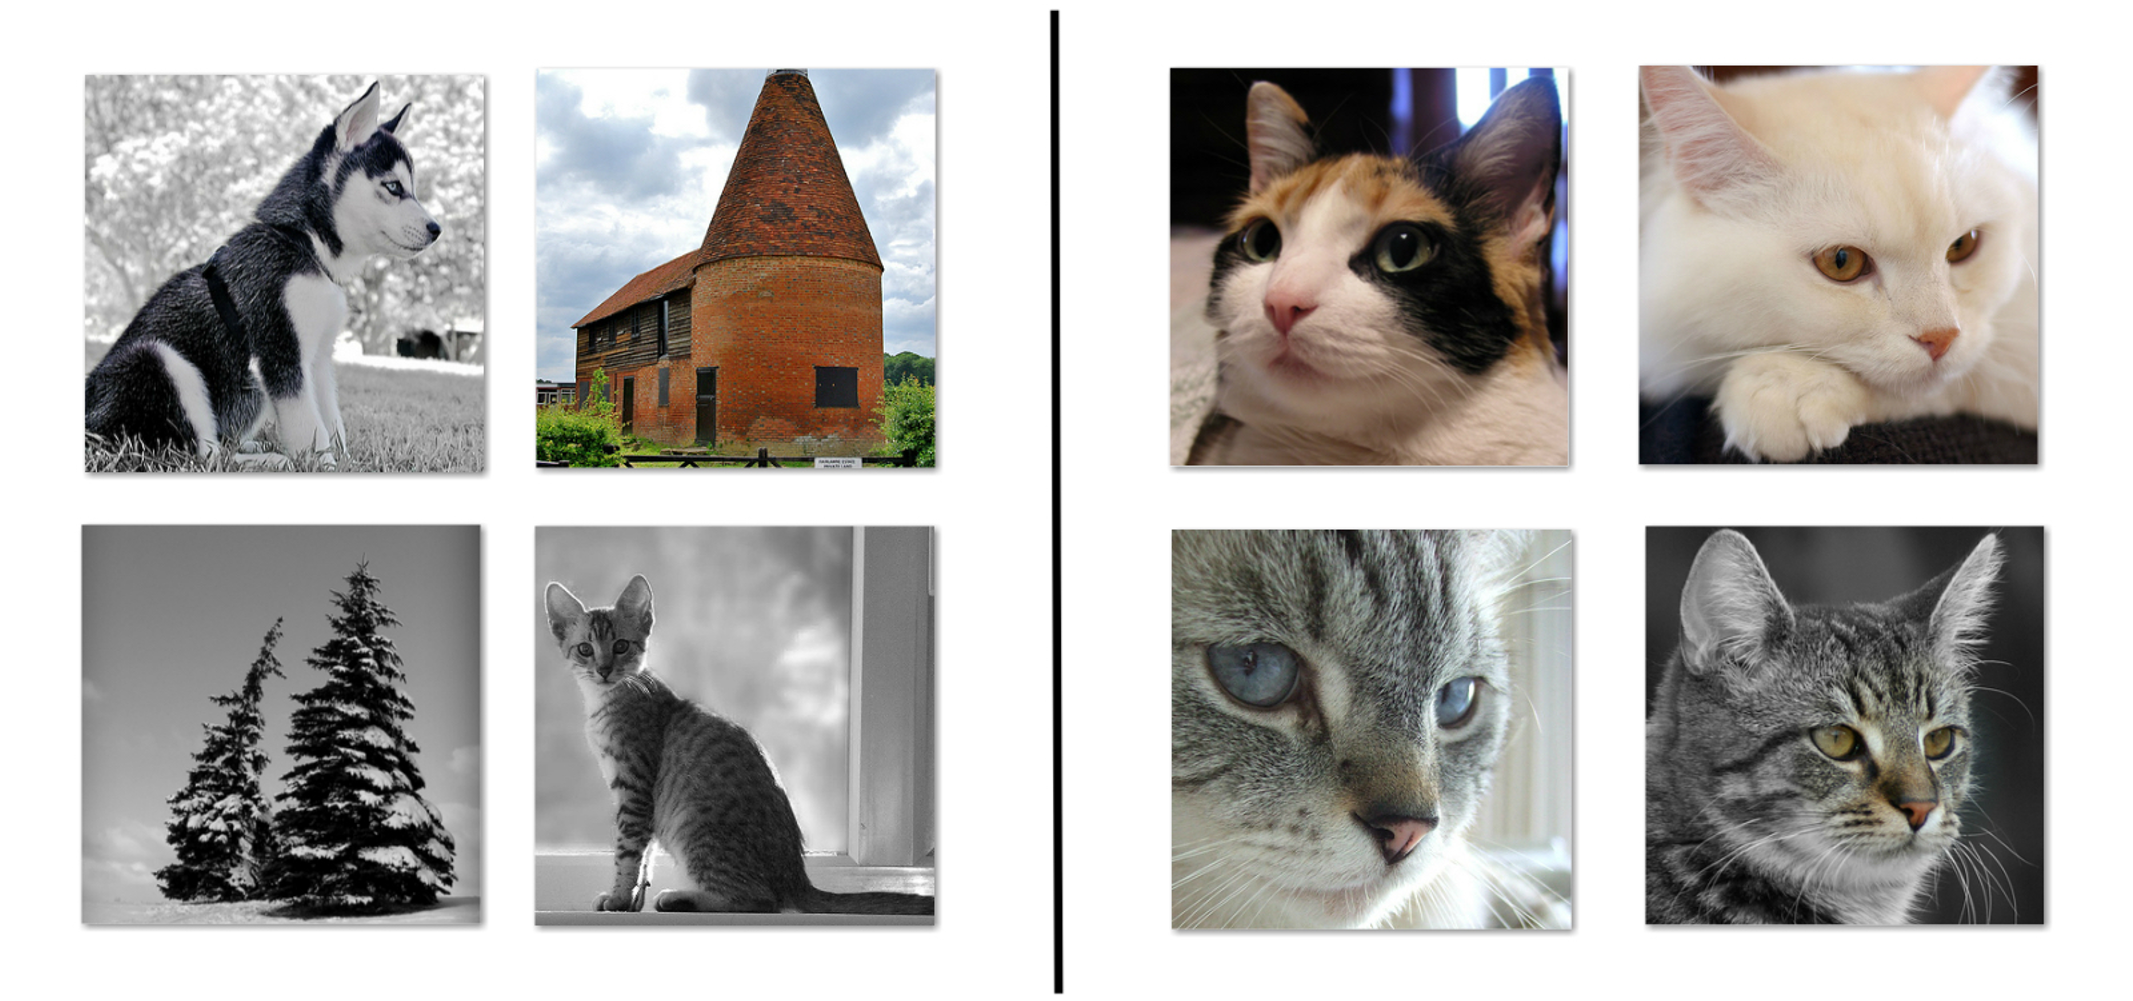
\includegraphics [scale=0.12] {twoGroups.png}
    \caption{Distinguishing dog, house, tree, cat in the left group is much easier than classifying the four cat types in the right, i.e., kitty cat, tiger cat, Angora cat, and Egyptian cat. }
    \label{fig:classEffect}
\end{figure}



%Instead, we observe that CNNs often have strong redundancy inside its structure, i.e., within feature maps, across channels, and across layers. Inspired by the loop perforation technique from source code optimization \cite{figurnov2016perforatedcnns}, we can speed up computation by skipping their evaluation in some of the positions. We further observe that different positions has different redundancy and we can select the hyper-parameter according to their influence over final accuracy. Based on these insight, we propose a framework, called \textit{perforation}, for selecting hyper-parameters in three levels; i.e., neuron-wise, channel-wise, and layer-wise, without any finetune for the new architecture and agnostic to the model architecture. While carefully hand-crafted architecture, SqueezeNet, achieves AlexNet-level accuracy with $50$x less parameters, perforation can reach $600$x reduction in parameters while also achieve AlexNet-level accuracy. Perforation is orthogonal to matrix factorization, matrix pruning, quantization, and group convolution, and can be combined with all for further optimization. When combined with runtime class skew, perforation can prune the model according to which classes appear in current environment and only maintain the important path for appearing classes.

In this paper, we present \textbf{SECS}, an efficient deep stream processing service. SECS efficiently detects and utilizes runtime class skew and prunes the candidate model according to the environment and the resource budget, as detailed in section \ref{SECS}. We carefully design a profiler to detect the class skew. Once the class skew is detected, the profiler will further decide whether the class skew is a hot class skew or a cold one. For cold class skews, probability layer is utilized to efficiently adapt the model towards the class skew during runtime with no overhead. If the class skew is marked a hot one, the profiler will aggressively optimize the model with class-specific pruning after the resource constraint is resolved. The adapted models will be stored in model bank and during runtime a scheduling model based on control theory will dynamically select the Pareto-optimal models under the available resource budget. Extensive evaluation shows that our system can potentially reduce the computation by xx times and memory consumption by xx times.

In summary, we make the following contributions:

\begin{enumerate}
  \item We identify an widely-existing environment information, class skew, which can both decrease resource consumption and increase accuracy.
  \item We bring up \textit{probability layer} to efficiently adapting all models to the class skew without any overhead and achieving an equal or better accuracy than finetuneing.
  \item We identify class skew dichotomy and bring up two modes, interpreation and compilation, to adapt the model with no overhead for cold class skews and prune aggressively for hot class skews to gain long-term benefit.
  \item We identify that some class groups are easier to classify while distinguishing some other class groups are harder and bring up \textit{class-specific pruning} to automatically select hyper-parameters according to the targetting classes without any finetuning during the selection process.
  \item We build a system, \textit{SECS} for efficient deep stream processing service. Extensive evaluation confirms its benefit is significant.
\end{enumerate}




\section{Motivation} \label{Motivation}
\subsection{Motivating applications}
Among the fastest growing applications, vision-based cognitive assistance applications and robotics visions are two representative categories.

As an example of cognitive assistance applications, smart glasses, Aira \cite{aria2018}, continuously recognizes surrounding environment and help the blind person with ordinary tasks, i.e. reading a handwritten note, navigating the grocery store, and even to run the Boston Marathon. To make it feasible, these smart glasses are expected to be lightweight and run at least several hours before recharging. 

On the other hand, robotic visions are expected to recognize objects automatically and work in the wild for days. For example, remote-controlled robotic animals are used by BBC \cite{bbc2018} to search specific animals and document secret lives of animals in the wild. Teleoperated robots \cite{landmine2018} are used for detecting and removing landmine in various environment. SpotMini \cite{spot-mini} are expected to handle objects, climbs stairs, and will operate in offices, home, and outdoors.

\paragraph{Common themes.} While these mobile platforms are resource-limited and latency-sensitive, CNN models with high resource consumption are still expected to be deployed on them, since CNNs has a much better performance than traditional approaches. The problem of tension is well- known, and existing methods of solving this problem generally trade accuracy for resource and speed. Now we want to make use of class skew to improve CNN models with both accuracy increasing and resource consumption decreasing. We will discuss about the features of class skew and how to utilize it efficiently in details next.

\subsection{Features of input and Opportunities}
The above applications all take input from the life-style environment. Such input exhibits class skew, since the activities of mobile devices show strong spatial and temporal locality. 

\paragraph{Temporal locality.} We can view the input stream as a continual camera feed. In the input stream, every frame differs only slightly from previous frames. Thus, the objects in frames usually keep appearing for a time period before the user moves to another scene. For example, a small group of people will appear frequently in a scenario of films, generally lasting for tens of minutes, and another group of people will not appear until the scenario has changed. The class skew appears frequently and provides chance to simplify CNN models. 

\paragraph{Spatial locality} It is common for humans to follow along recurrent trajectories, for example, due to their regular social activities or frequenting a favorite park from time to time. Therefore, there is some level of recurrence of the scenes obtained as part of those activities. Through these repeating scenarios, same class skew will also keep appearing, which make it a feasible choice to optimize CNNs towards the class skew.

The existence of strong temporal and spatial locality indicates the existence of class skew. Experiments on videos of day-to-day life from Youtube \cite{shen2016fast} shows that $10$ objects comprised $90$\% of all objects in $85$\% time. Utilizing class skew will both increase accuracy and decrease resource consumption, as detailed in section \ref{evaluation}. 

We further observe the existence of class skew dichotomy, which means that some class skews appears in the future, called hot class skew, while other class skews never appear again or appear seldom, called cold class skew. Inspired by techniques from source code, this dichotomy motivates us to implement two different levels of optimization with different overhead on hot and class skew, called the compilation and interpretation. Specifically, class-specific pruning can be conducted on hot class skews to achieve extra benefit.


\subsection{Challenges}
In order to utilize class skew more efficiently, we need to deal with class skew switch and explore how to conduct class-specific pruning with low overhead. 

It is obvious that class skew switches frequently as time goes, i.e., every $10$ minutes. Dealing with this phenomenon is hard because it is infeasible to pre-train a model for every class skew during the deployment time, due to the mind-bogglingly huge number of class combinations. In existing works \cite{\cite{han2016mcdnn, shen2016fast}}, a general model handling all possible classes will be trained at the deployment and once the class skew is detected during runtime, the model will be adapted correspondingly. Specifically, the number of nodes in the softmax layer will be reduced and the last few layers will be finetuned during runtime towards the class skew under the direction of transfer learning \cite{doersch2015unsupervised, noroozi2016unsupervised, oquab2014learning, yosinski2014transferable}, which consumes energy and memory intensively. 

The challenge of class-specific pruning resides in the obstacle of comparing the performance of various hyper-parameters. Class-specific pruning requires to select the simplest model with least layers, channels, and neurons for a given group of classes. During this process, the relative importance of different layers, channels, and neurons on accuracy needs to be compared and the parameters with least influence should be removed. However, to get the exact performance, training the new model cannot be avoided while it is unaffordable to do so for each new architecture. Existing papers hand-select architectures, which is not automatical and only test a small space of hyperparameters, i.e. $2$ or $4$ convolutional layers, $32$ or $64$ neurons in each layer, as detailed in section \ref{relatedWork}.


We address these challenges by probability layer, an efficient model adaption algorithm, and perforation, an automatic class-specific pruning methods with no finetuning during the process of selection hyper-parameters. Further, we designed a real-time image classification framework, SECS, to automatically detect and utilize class skew, as well as select the Pareto-optimal models under available resource budget.
























\section{SECS System Design} \label{SECS}
\subsection{Overview}

\begin{figure} 
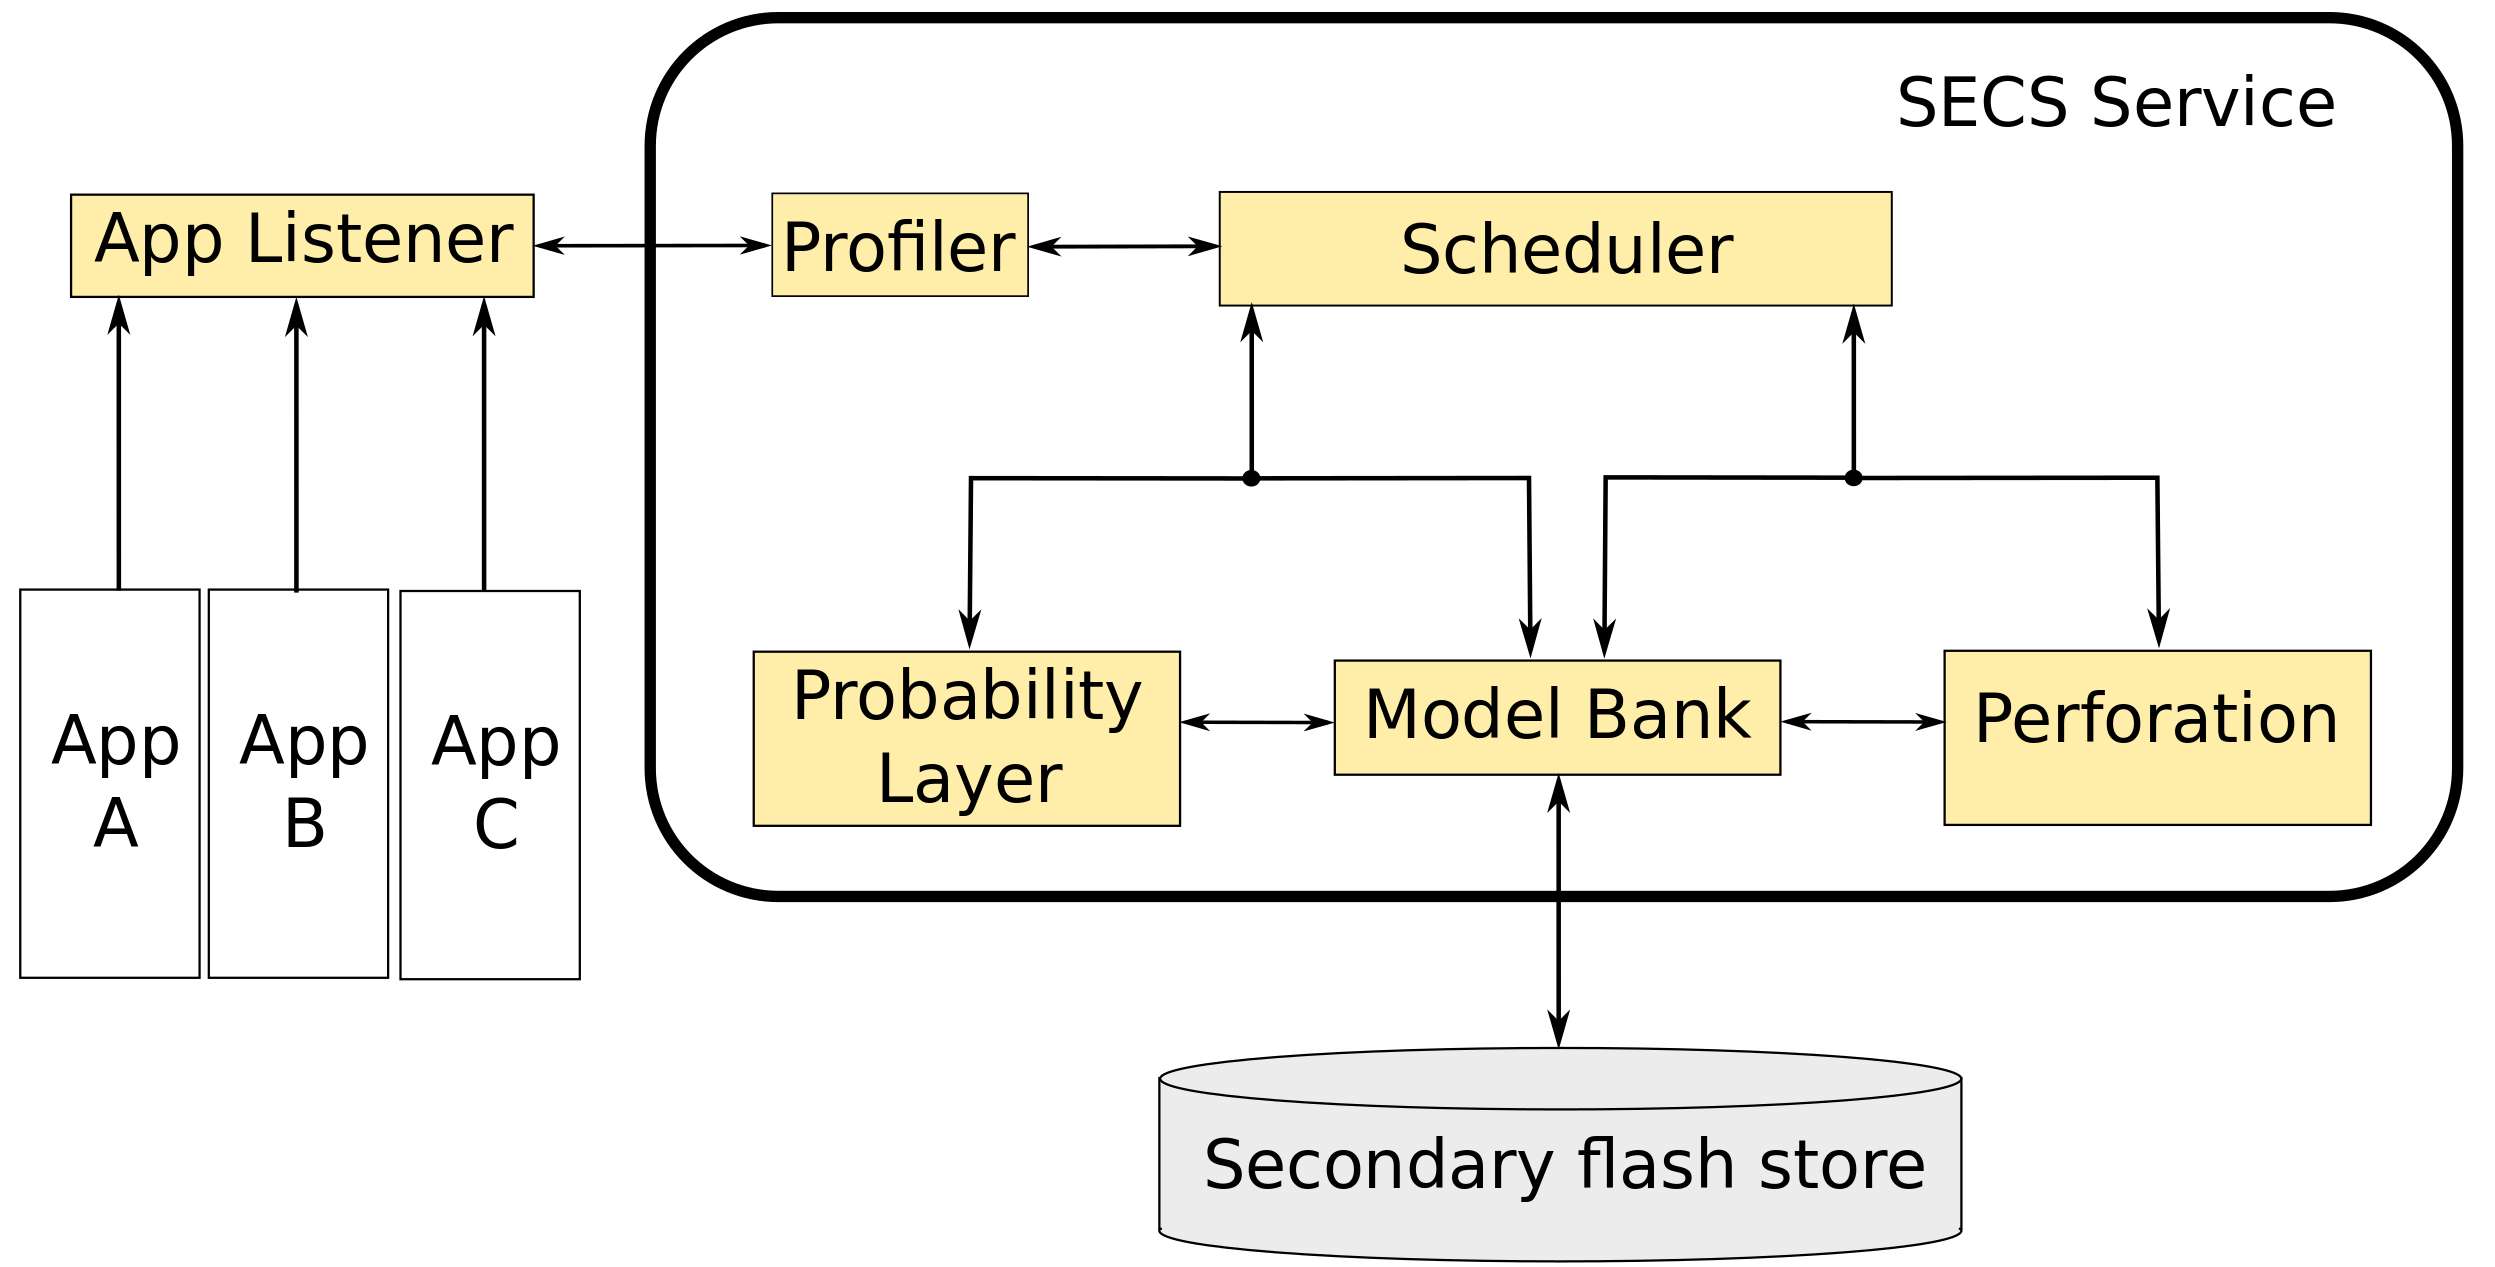
\includegraphics[scale=0.095]{architecture.png}
\caption{System architecture.}
\label{fig:Architecture}
\end{figure}

SECS is a real-time deep stream processing system utilizing class skew efficiently and conducting class specific pruning automatically, as detailed in Figure \ref{fig:Architecture}. The \texttt{AppListener} maintains a threadpool, summarizes the requests from upper-level applications into a stream, and forwards the stream into \texttt{profiler} for further procedure. During runtime, the \texttt{profiler} maintains current class distribution and effectively detect class skew. Once class skew is detected, the \texttt{profiler} will either call existing adapted model from \texttt{model bank}, or require the \texttt{probability layer} to efficiently adapt the model. The classification results will be feed back to \texttt{profiler} which will both respond the \texttt{AppListener} and update class skew. During cold time, the \texttt{profiler} will check whether a class skew has appeared more frequently than a pre-defined threshold, and call \texttt{perforation} to generate class-specific pruned models for more optimized classification in the future. We discuss the individual steps next.






\paragraph{Notation}
CNN can be viewed as a feed-forward multi-layer architecture that maps the input images $X$ to a vector of estimated probability for each class $\vec{p} = (p_1, p_2, ..., p_n)$, where $n$ is the number of classes and $p_i = P(i|X)$ is the estimated probability $p_i$ for the label $i$ given the input image $X$. In particular, the image feature maps in the $l$-th ($1 \leqslant l \leqslant L$) layer can be denoted by $\mathcal{Z}_l \in \mathbb{R}^{H_l \: \times \: W_l \: \times \: C_l}$, where $H_L$, $W_l$, $C_l$ are the dimensions of the $l$-th feature maps along the axes of sptial height, spatial width, and channels , respectively. $L$ denotes the number of convolutional layers. Individual feature maps in the $l$-th layer could be denoted as $\mathcal{Z}_l^{(k)} \in \mathbb{R}^{H_l \: \times \: W_l}$ with $k \in [1, \:2, \: \dots \:, C_l]$. The individual output feature map $\mathcal{Z}_l^{(k)}$ of the $l$-th convolutional layer is obtained by applying the convolutional operator ($\ast$) to a set of input feature maps with the corresponding filter $\mathcal{W}_l^{(k)} \in \mathbb{R}^{d \: \times \: d \: \times \: C_{l-1}}$, i.e.,
\begin{equation}
    \mathcal{Z}_l^{(k)} = f(\mathcal{Z}_{l-1}^{(k)} \ast \mathcal{W}_l^{(k)}),
\end{equation}
where $f(\cdot)$ is a non-linear activation function. Further, the $l$-th layer can be written as
\begin{equation} \label{eq:1}
    \mathcal{Z}_l = f(\mathcal{Z}_{l-1} \ast \mathcal{W}_l)
\end{equation}
where $\mathcal{W}_l \in \mathbb{R}^{C_l \: \times \:   d \: \times \: d \: \times \: C_{l-1}}$.



\subsection{Probability Layer}
In this section, we introduce the probability layer, which can adapt the general model towards the class skew without any overhead.

\paragraph{Key Assumption.} 
The main difference between the proposed layer and the original CNNs is that we take the environment information into consideration. In original CNNs, the prediction for each image will be made individually, assuming a sequence of images is independent and identically distributed (\textit{i.i.d}). However, in real life, this assumption does not hold and strong temporal and spatial locality may exist. Instead, we assumes class skew exists, which means the number of classes and class types are fixed during a time period. Meanwhile, it is still possible that the class skew switches to another class skew after a few minutes, which can be detected and handled by the profiler, as detailed in section \ref{profilerSection}. Further, we assume the existence of a model classifying all possible classes, called the \textit{general model}. This assumption is reasonable because modern CNNs can be trained to classify thousands of classes \cite{krizhevsky2012imagenet, simonyan2014very, szegedy2015going, he2016deep, huang2017densely}.



\begin{figure}[t]
\begin{subfigure}{.23\textwidth}
  \centering
  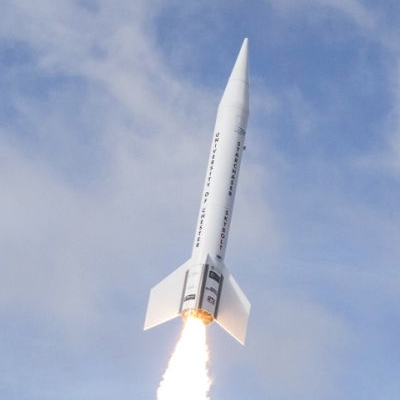
\includegraphics[width=\textwidth]{rocket.png}
  \caption{Rocket}
  \label{fig:sub2}
\end{subfigure}
\begin{subfigure}{.23\textwidth}
  \centering
  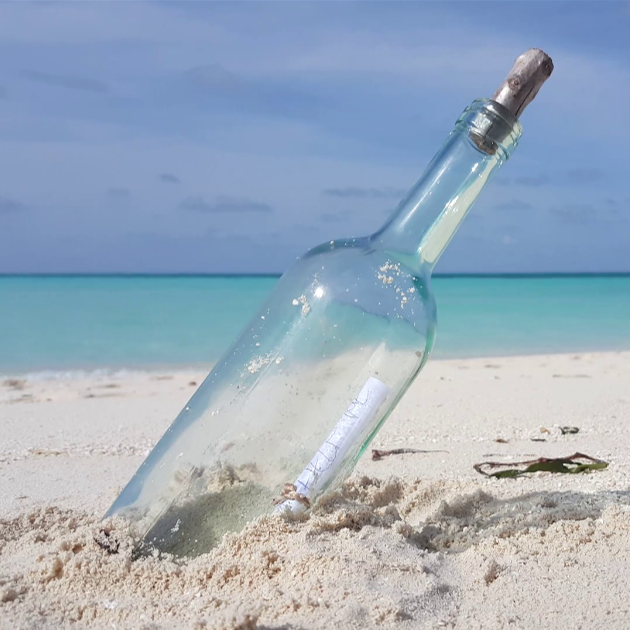
\includegraphics[width=\textwidth]{bottle.png}
  \caption{Bottle}
  \label{fig:sub3}
\end{subfigure}
\label{fig:exampleSimilar}
\caption{Examples of similar classes.}
\end{figure}





\paragraph{Intuition.}
Probability layer helps by using environment information that original CNNs does not use. When human recognizes an object, both vision and environment information will be used, i.e., what we have seen recently and which objects may appear here. However, CNNs can only make use of visual information while discarding environment information, which makes it extremely difficult to distinguish classes with similar appearance. For example, Figure \ref{fig:sub2} and Figure \ref{fig:sub3} shows images for bottle and rocket respectively. It is hard to distinguish these two classes only from images while environment information can easily rule out rocket in most scenarios. 

Figure \ref{fig:intuition} gives intuition on how probability layer utilize environment information. In Figure \ref{fig:intuition}, the lower row represents the outputs from softmax layer and the upper row represents the probability layer. The orange nodes stand for the classes with high predicted probability in softmax layer and the red nodes stand for the suggestion from the environment. The prediction from probability layer will be selected from the intersection of the set of red nodes and orange nodes, which rules out confusing classes for CNNs. The intersection will not be empty since the red nodes are the classes detected by the general model frequently during the recent time period.
%how to select general model?


\begin{figure}
  \centering
  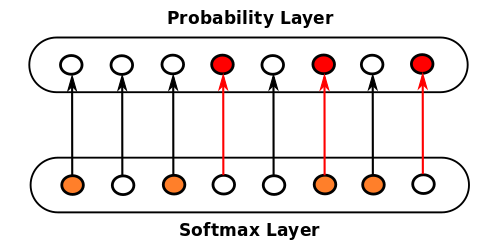
\includegraphics[width=.45\textwidth]{intuition.png}
\caption{Intuition on how probability layer and softmax layer take effect together.}
  \label{fig:intuition}

\end{figure}

\paragraph{Approach. } Probability layer is an extra layer after the CNN model, rescaling the output of softmax layer. Rescaling is a topic in statistics \cite{saerens2002adjusting}. To the best of our knowledge, we are the first to discuss rescaling in CNN context. The outputs of original CNNs predict the probability for each class and the probability layer will adjust this prediction based on the difference of class distribution in training and testing dataset. In particular, for classes with different distributions in training and testing dataset, the probability layer will rescale the corresponding outputs from softmax layer according to the difference in distribution. For other classes with same distribution in both training and testing dataset, the outputs of the proposed layer are equal to the outputs of the softmax layer. 


The probability layer will take as input the originally predicted probability, class distribution in training dataset, as well as the distribution in testing dataset, and output a vector for the rescaled prediction. The first input is the prediction vector $\mathbf{P}(\cdot|X)$ from the softmax layer, which represents the originally predicted probability for each class from the original CNNs. The second input is a vector of class distribution $\mathbf{P}(\cdot)$ in training dataset and the third one is a vector of class distribution $\mathbf{P}_t(\cdot)$ in testing dataset. The probability layer will rescale the predicted probability in $\mathbf{P}(\cdot|X)$ element wisely and produce as output a vector $\mathbf{P}_t(\cdot|X)$ for the rescaled prediction of each class.

Formally, let the outputs of CNNs with and without rescaling are
\begin{equation}
    P_t(i|X) = \frac{P_t(X|i) \cdot P_t(i)}{P_t(X)}
\end{equation}
and
\begin{equation}
    P(i|X) = \frac{P(X|i) \cdot P(i)}{P(X)}
\end{equation}
respectively. Here $P_t(i)$ means the class distribution in testing dataset and $P_t(i|X)$ represents the predicted probability for class $i$ after the probability layer. We assume that $P_t(X|i)$ equals $P(X|i)$ approximately, where $P(X|i)$ is the distribution of image data for class $i$. This assumption makes sense since, for a class $i$, the selection of input x is random. Through transforming equation $4$ and equation $5$ as well as utilizing $P_t(X|i) = P(X|i)$, we can derive that 
\begin{equation}
    P_t(i|X) = \frac{P_t(i)}{P(i)}\cdot P(i|X) \cdot P(X) 
\end{equation}. Considering $\sum_{i=1}^n P_t(i|X) = 1$, we can get the rescaling formular as
\begin{equation}
    P_t(i|X) = \frac{\frac{P_t(i)}{P(i)} \cdot P(i|X)}{\sum_{j=1}^n \frac{P_t(i)}{P(j)} \cdot P(j|X)}
\end{equation}


To give probability layer the ability to detect new classes, we choose not to rescale the outputs from softmax layer when the original model has strong confidence in its prediction and set the formula of probability layer as
\begin{equation} \label{eq: recover}
    P_t(i|X) = \frac{\frac{P_t(i)}{P(i)} \cdot P(i|X)}{\sum_{j=1}^n \frac{P_t(i)}{P(j)} \cdot P(j|X)} \cdot I_{\{P(i|X) < \omega\}} + P(i|X) \cdot I_{\{P(i|X) >= \omega\}} 
\end{equation}
, where $\omega$ is the threshold above which we should trust the original prediction and $I_X$ is the indicator function such that
$I_X(x) \delequal \; $if $x\in X$, return $1$, otherwise return $0$.
If a model have a strong confidence in its prediction, the accuracy would be much higher than the model's average accuracy. Our experiments show that CNNs will give most of the images high predicted probability and the accuracy of these images will exceed average accuracy a lot. Probability layer helps when the original model is confused on the prediction and will not interfere the decision when the original model has confidence in its prediction.




\subsection{Class-specific pruning}
In this section, we introduce class-specific pruning, which can optimize the model architecture based on which classes will appear. Then, we bring up perforation to speed up class-specific pruning, which is a pruning method on three levels, i.e. neuron-wise, channel-wise, and layer-wise.


\paragraph{Class-specific pruning.} 
We observe that some groups of classes are much harder to classify than others, as indicated in Figure \ref{fig:classEffect}. For example, it is much easier to classify house, cat, dog, and tree than distinguishing four different cat species. In fact, distinguishing four different cat species requires expertise in cat species and carefully check on subtle features, i.e. ear size, tail length, coat patterns, and sometimes even personality \cite{cat2018}. Through a series of experiments, we found that classes with low similarity have much higher testing accuracy than classes with high similarity even if the model architecture and the number of classes remain unchanged. Specifically, using a CNN model with 4 convolutional layers and 3 fully connected layers, the accuracy is only 31.49\% to classify baby, boy, girl, man, woman from CIFAR100 while the accuracy would increase to 66.5\% when classifying bottles, bowls, cans, cups and plates. Following along this line of thought, with the same targetting accuracy, models could consume less resource to classify a group of classes with high difference. 

To do so, during the hyper-parameter selection process, instead of the original dataset with all possible classes, a specialized dataset with only targetted classes are used and the accuracy on the specialized dataset is treated as standard to select the model with least resource consumption and best performance. Class-specific pruning is challenging since hyper-parameter selection process is time consuming. For every new sets of hyper-parameters, the model need to be retrained, which may take days or even weeks. Perforation is brought up to reduce the overhead, as detailed in section \ref{perforation}.

Also note that class similarity is orthogonal to number of classes since number of classes consider how many classes have appeared in a scenario and class similarity considers how similar the group of classes are to each other, which is orthogonal to number of classes. Thus the class specific pruning could be used simultaneously with probability layer.


\subsubsection{Perforation} \label{perforation}




Perforation could be used both as general pruning technique and class-specific pruning technique. As a general pruning technique, perforation can produce an automtically selected model with 600x less parameters with AlexNet-Level accuracy, while SqueezeNet \cite{iandola2016squeezenet}, a hand-selected architecture, can only use 50x less parameters with AlexNet-Level accuracy. As a class-specific pruning methods, the automatically generated model can achieve the same accuracy with further 20\% less resource consumption to classify house, cat, dog, and tree than distinguishing four different cat species, see section \ref{evaluation}. (VALUES TO BE CHANGED)



\paragraph{Intuition. } The motivation for perforation is the observation that in the hyper-parameter selection process, we only need the relative performance of models instead of the exact accuracy. Inspired by techniques from the source code optimization \cite{figurnov2016perforatedcnns}, we use perforation to recover the skipped positions after we delete the most unsalient positions towards the accuracy. The positions here could be layer-wise, channel-wise, or neuron-wise. 



\paragraph{Layer-wise perforation.}
We introduce a global mask $M$ to temporally mask out unsalient filters in each iteration based on a pretrained model. Therefore, equation \ref{eq:1} can be rewritten as:
\begin{equation} \label{eq: 2}
    \mathcal{Z}_l = M_l \cdot f(\mathcal{Z}_{l_1} \ast \mathcal{W}_l), \ \ \  s.t. \: l = 1,\: 2, \: \dots, \: L,
\end{equation}
where $M_l \in \{0, 1\}$ is a mask with a binary value. $M_l = 1$ if the $l$-th layer is salient, and $0$ otherwise. $\cdot$ denotes the point-wise product. By masking out certain layer as zero, we can view it as skipping the computation of this layer. This operation will make the input to the next layer to be zero and requires finetuning to continue. Instead, we perforate the skipped layer by concatenating same number of channels from previous layers, which can maintain the input tensor size to the next layer and continue prediction without finetuning. Thus equation \ref{eq: 2} can be rewritten as:
\begin{equation}
    \mathcal{Z}_l = g(m_l, f(f(\mathcal{Z}_{l_1} \ast \mathcal{W}_l)), Z_{l-1}), \ \ \  s.t. \: l = 1,\: 2, \: \dots, \: L,
\end{equation}
where $g(x,y,z)  \delequal \; $if $x = 1$, return $y$, otherwise return $z$.

The problem to prune the most unsalient layers until there are only $K$ layers can be rephrased as an optimization problem:
\begin{equation*}
\begin{aligned}
& {\text{min}}
& & L(Y, h(X; W, m)) \\
& \text{s.t.}
& & ||m||_0 \leq K
\end{aligned}
\end{equation*}
To solve this problem, we provide a heuristic algorithm. In each round, we will remove the layer with smallest negative effect on the final accuracy. Each round can be seperated into many steps and in each step we will remove a single layer while keeping all the other layers. Since perforation is used to recover the feature map size to the layer after the skipped layer, the computation can continue and the final accuracy is still available. Thus in each step, we can get the accuracy after removing the corresponding layer. After iterating through all layers, we can get which layer has smallest negative effect on the final accuracy and remove this layer.

\paragraph{Channel-wise perforation.} Channel-wise perforation could be done in a similar approach with layer-wise perforation. Instead of masking out the whole layer, we adopt a finer granularity with a vector $m_l = \{0,1\}^{C_l}$ as channel-wise mask. The equation \ref{eq:1} can be rewritten as:
\begin{equation} \label{eq: 3}
    \mathcal{Z}_l = f(\mathcal{Z}_{l_1} \ast (m_l \odot \mathcal{W}_l) ), \ \ \  s.t. \: l = 1,\: 2, \: \dots, \: L,
\end{equation}
where $m_l = 1$ if the $l$-th filter is salient, and $0$ otherwise. $\odot$ denotes the channel-wise product. By masking out certain channels as zero, we can view it as skipping the computation of this layer. For the reason of continue computation, we perforate the skipped channels by previous channels. Similar to the heuristic algorithm in layer-wise perforation, we can prune channels in a one-by-one approach.

\paragraph{Neuron-wise perforation.} We choose to increase strides to skip neurons instead of using a mask to identify important neurons in each feature maps. The reason is that, as indicated in \cite{aklaghi2018snapea, buckler2018eva, hegde2018ucnn}, this process may introduce irregularity in the computation of neurons and overhead on computation will be introduced. By increasing strides, we can still skip some neurons while there are mature implementation of increasing strides.

%\paragraph{Speed up perforation}
%In the procedure of pruning, we generate a cascade of models with decreasing accuracy. When redundancy in architecture is abundant, a single step in the perforation may only decrease the accuracy by less than $0.1$\%. However, we do not require a too fine-grained cascade since it indicates a larger number of models and more disk consumption. Instead, SECS service would require the user to define a threshold on the required granularity and adjust the perforation rate during the pruning procedure to maintain a cascade with required granularity (=1\% in our implementation). 

%We utilize control theory to speed up perforation. When the accuracy remains similar, we will increase the perforation speed, i.e. decrease more channels, layers or increase more strides during the same perforation step.

\paragraph{Search suitable architectures.}
During the procedure of perforation, we can generate a cascade of models with decreasing resource computation and performance. To find the model with targetted accuracy, we do not need to finetune all models. Instead, based on the property of decreasing accuracy, we can test the models in a binary search approach, which would only take logarithm times.

\paragraph{Discussion on reducing resolution}
Reducing resolution has been reported as an effective approach in optimizing architecture \cite{krizhevsky2009learning, fu2017look, howard2017mobilenets}. Reducing resolution indicates the proportional reduction in feature map sizes in all layers and thus both reduces computation and memory consumption proportionally. However, reducing resolution forces the reduction in feature maps sizes in a uniformly way across all layers. We argue that reducing uniformly is infeasible since different positions in the architecture has different degree of redundancy. Instead, perforation could reduce feature map sizes, channel numbers, and layer numbers according to the redundancy in different positions and prune the architecture correspondingly, which would introduce more optimization with less penalty in accuracy. Actually, reducing resolution is equivalent to add a pooling layer before the whole architecture or increase strides in the first layer, which is covered by perforation and could be selected when feasible.

Also note that in MobileNet \cite{howard2017mobilenets}, reducing resolution is utilized by adding an extra hyper-parameter selected by hand, which becomes an obstacle for users who are not familiar with CNN architectures. Instead, perforation selects in an end-to-end automatic way and hide procedures from users.



\subsection{Profiler} \label{profilerSection}
Profiler detects class skew and makes a series of decisions on whether or not a class skew exists, which model to run, and whether a class-specific pruning is necessary or not. We phrase the class skew detection problem as a oracle Bandit problem \cite{auer2002finite, lai1985asymptotically} and utilize WEG algorithm \cite{shen2016fast} to solve it efficiently.

Let denote a stream of images to be classified as $x_1, \: x_2, \: ...,\: x_i, \: ... \in X = \mathbb{R}^n$ and the corresponding true labels as $y_1, \:y_2, \:...,\:y_i, \:... \in Y = [1, ..., k]$. Assume a partition $\pi: I^+ \rightarrow I^+$ over the stream exists, where each partition maintains a distribution $T_{\pi(i})$ and the image $(x_i, y_i)$ is drawn randomly from distribution $T_{\pi(i)}$. Here, the overall series is an abruptly-changing and piece-wise stationary distribution. At test time, neither true labels $y_i$ nor partition $\pi$ is known. Also we do not have any assumptions on how long a stationary distribution exist. The task of profiler is to detect the stationary distribution when it appears and switch to another stationary distribution when it switches.

The emergence and disapperance of class skew can be detected by the WEG algorithm, as shown in the existing work \cite{shen2016fast}. Since the duration of class skew cannot be decided easily, we detect the class skew in a windoed style, as detailed by WEG() in algorithm \ref{alg: algorithm}, line \ref{alg: WEG}. Every $w_{min}$ frames form a window and we can run the full model on each frame and record the distribution in these $w_{min}$ (= 30) frames. We can further compare the record in $S_j$ and $S_{j-1}$. If the difference in appearance times is less than a threshold $\pi_r$ (=2), we conclude that the previous epoch is continuing and use their concatenation as the estimation of class skew. 



\begin{algorithm} 
 \small
 \caption{Windowed e-Greedy (WEG)}
  \begin{algorithmic}[1]
    \Function{WEG}{$ $} \label{alg: WEG}
        \For{$i$ in $1, ..., w_{min}$}
            \State $y_t \leftarrow h(t)$
            \State $S_j \leftarrow S_j \oplus [y_t]$
        \EndFor
        \If{$|| S_{j-1}, S_j|| \leq \pi_r$}
            \State $S_j \leftarrow S_{j-1} \oplus S_j$
        \EndIf
        \State \Return $S_j$
    \EndFunction
  
    \Function{Scheduler}{$i, r$}  \Comment{$r$ denotes current class skew} \label{alg: scheduler}
        \State $M \leftarrow collectModel(r)$
        \State $EPF \leftarrow RemainEnergy() / (RemainingTime() \ast F) $
        \State $a, m \leftarrow chooseModel(EPF, r, M)$  
        \State $execute(i,m)$        
    \EndFunction
\end{algorithmic}
 \label{alg: algorithm}

\end{algorithm}


The detected class skew will be processed by the profiler, as detailed by line \ref{alg: scheduler}. The profiler will import the class-specific pruned models in the model bank if available. If no class-specific pruned model is available, the profiler will call the probability layer to adapt the models immediately. These candidate models will serve further decisions along with recorded properties, i.e. energy and memory consumption, as well as accuracy. Then the profiler estimate the energy per frame by the average of available resource over remaining times and frames. Finally, $ChooseModel$ will return the most accurate model under current resource budget. 

While original WEG algorithm \cite{shen2016fast} builds a complex scheduling model for trade-off between accuracy benefit and cost from runtime finetuning, our profiler does not need it, since the probability layer produces adapted model efficiently and class-specific pruned model are also not produced during runtime. In addition, the detection of change in class skew can be achieved by equation \ref{eq: recover}, since the probability layer will not interfere the decision when the original model has confidence in its prediction.




Further, the number of appearance for this class skew will be increased by one and compared with a threshold $\pi_h$. If the class skew has appeared frequently, it will be marked by profiler as the hot class skew and class-specific pruning will be called after the resource constraint on the mobile platform is resolved, i.e. being connected to power and starting to recharge.





\section{Implementation} \label{implementation}
We implement SECS as a end-to-end classification service with Tensorflow \cite{tensorflow2015-whitepaper}. 


\subsection{Image classification service}
\paragraph{Probability layer.}
We build probability layer by adding a single extra layer after the original model. The probability layer could be implemented as a variable using \textit{tf.get\_variable} with dimension \textit{1xn}. The probability layer will be initialized with the runtime class skew recorded by \texttt{profiler}, which is freely available and no overhead is introduced. The sum of this variable and the original softmax layer will replace the original softmax layer and used as the classification results. 

\paragraph{Perforation.}
There are three levels of perforation, i.e. neuron-wise, channel-wise, and layer-wise. Generally, we speedup computation by skipping several carefully selected positions. The reduced feature map sizes or number of channels will obstacle the forward computation in CNNs. Perforation is used to make up the holes that has been skipped using values from adjacent positions. 

Specifically, we implement neuron-wise perforation by increasing strides to reduce computation and use interpolation methods to recover the feature map sizes. By default, \textit{tf.image.resize\_images} and nearest neighbor algorithm is used for interpolation. 

To implement channel-wise perforation, we maintain a global 0-1 mask for all channels indicating whether or not keep the specific channels according to their importance towards accuracy. After masking out the channels, we fill the hole with adjacent channels. \textit{tf.split} can split tensors channel-wise effectively. These splited tensors can be concatenated using \textit{tf.concat} to recover the original number of channels and enable the forward computation with original weights. Layer-wise perforation could be implemented in a similar approach.




\paragraph{Model bank.}
All the generated models are stored in model bank. Each entry contains the status of a single model, including whether it is a general model or class-specific pruned model, required computation and memory, as well as the accuracy. \textit{N/A} indicates no class skew used in the model. The model bank will support the runtime decision from \texttt{profiler} and only models at the Pareto-optimal bound will be selected for service.



\subsection{Sharing}
It has been identified by existing works \cite{guo2018potluck, jiang2018mainstream} that multiple applications could process same input stream concurrently. Thus the same classification results could be shared among all applications instead of repeating the computation by each applications. To do so, we build an interface \textit{AppListenser} to get request from all applications and feed back same results to everyone. 



\paragraph{AppListener.}
As the interface, \texttt{AppListener} receives messages from applications containing the input images and required accuracy. To synchronize the requests from all applications, the input images received within a time period will be averaged into a single one and all related requests will get the same results. As indicated by \cite{guo2018potluck, jiang2018mainstream}, the choice of this threshold represents a tradeoff between resource efficiency and accuracy. By default, we choose the threshold as a half second.

\subsection{APIs and patches to the application code}
To simplify the usage of SECS service, the user only need to use the interface \textit{requireAccuracy()}, providing required accuracy, and \textit{requireTime()} indicating how long the system are expected to run. Both classification and pruning will be done by SECS service automatically. In addition, an interface, \textit{register()}, is designed for applications to register in the SECS system.








\section{Evaluation} \label{evaluation}

\subsection{General setup}



We implemented probability layer on DenseNet \cite{huang2017densely} and evaluated the CNN model with probability layer, i.e., \textit{PCNN}, on specialized datasets with various number of classes and class distribution. We choose DenseNet as the base model since it is the state-of-the-art and has similar results with other state-of-the-art models, i.e., GoogLeNet \cite{szegedy2015going} and ResNet \cite{he2016deep}. We reimplemented the DenseNet on Tensorflow \cite{abadi2016tensorflow} and trained the model on CIFAR100 \cite{krizhevsky2009learning} from scratch. The \textit{specialized dataset} is generated from CIFAR100 \cite{krizhevsky2009learning}, which originally has $100$ classes with equal weight. 

\textbf{Transfer Learning.} Following the published practice \cite{doersch2015unsupervised, han2016mcdnn, oquab2014learning, shen2016fast, yosinski2014transferable}, all fully-connected layers after convolutional layers are finetuned on the generated dataset with same class distribution as the testing dataset. To eliminate the effect of the epoch, we used three different epochs, i.e., $1$, $5$, and $30$. The maximum epoch is $30$ because latency and energy efficiency are considered.

\subsection{Class effect}
We explore the effect of class combinations and compare the performance of probability layer and transfer learning on various class combinations. Fixing the number of classes as two, we randomly selected five class combinations and compare the original model, model after transfer learning, and the model with probability layer, see Figure \ref{fig:classEffectExamples}. We see that with the same model, different class combinations may have dramatically different accuracy. While the original model can achieve a accuracy as 83\% for classifying chair and cup, the accuracy for beaver and bear is only 52.5\%. We can also observe that both transfer learning and probability layer can bring in benefit no matter which two classes compose the dataset while probability layer generally performs better than transfer learning. In the randomly selected five class combinations, probability layer can provide an additional benefit of $2.16\%$ on average.

Figure \ref{fig:classEffectSummary} gives a summary of the performance of all three models on the specialized dataset with two and five classes. The figure shows the result from $100$ randomly selected class combinations. We see that, on the original model, while the average accuracy for classifying two classes is $70\%$, the minimum accuracy could be $45\%$ and the maximum accuracy can reach $83\%$, which shows that the accuracy of classifying two classes could change dramatically even using the same model. This observation also holds for transfer learning and probability layer. We can also note that the average accuracy of probability layer is much higher than transfer learning. 

\begin{figure}[t]
    \begin{subfigure}[b]{0.235\textwidth}
        %\centering
        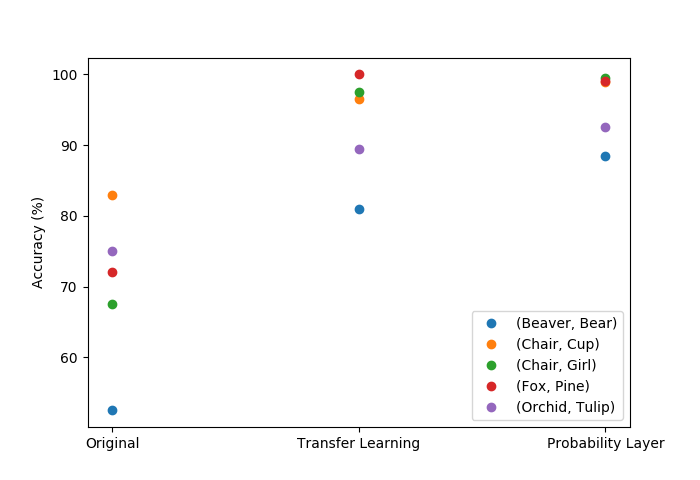
\includegraphics[width=\textwidth]{classEffectLine.png}
        \caption{Concrete examples}
        \label{fig:classEffectExamples}
    \end{subfigure}
    \begin{subfigure}[b]{0.235\textwidth}
        %\centering
        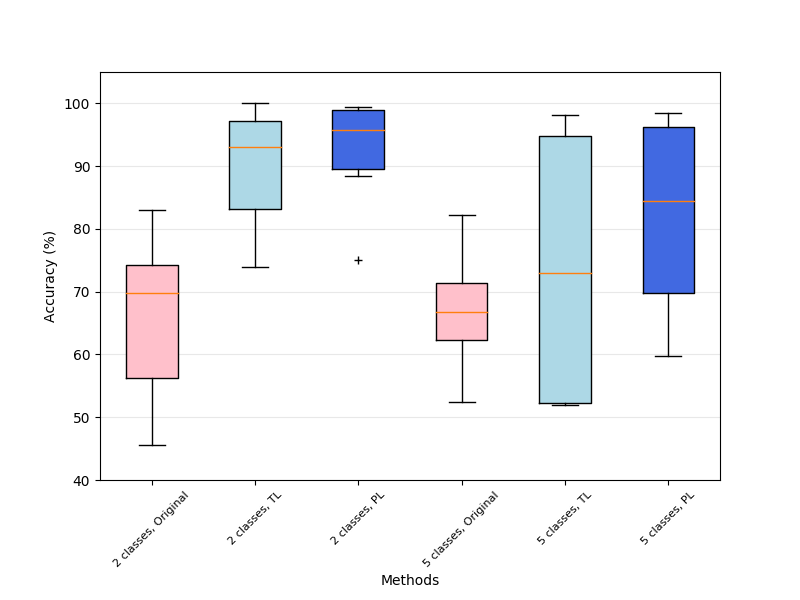
\includegraphics[width=\textwidth]{classEffect.png}
        \caption{Summary of class effect}
        \label{fig:classEffectSummary}
    \end{subfigure}
    \caption{Class effect on the original model, the model after finetuning, and the model with probability layer.} \label{fig:classEffect1}
\end{figure}
\subsection{Results on specialized datasets with only majority classes}

% Third paragraph: Experiment setting
We explore probability layer's ability on making use of environment when there are only a few majority classes. For each number of classes, we randomly sampled $100$ subsets of classes and present the average accuracy in Figure \ref{fig:PLvsRetrain}. We see that significant benefit has been achieved by probability layer for all number of classes. When there are 5 classes, an increase of more than $20\%$ can be achieved without any finetuning. Another point worth noting is that the benefit diminishes gradually as the number of classes increases. Even if there are $40$ classes, a benefit over $10\%$ could still be observed. This shows a significant advantage over previously published results \cite{shen2016fast}, in which no benefit exists when there are more than $15$ classes.
 
We compare our results with transfer learning in Figure \ref{fig:PLvsRetrain}. For every specialized dataset, we finetune the model for $5$ rounds on a training dataset with the same class combinations and class distribution as the testing dataset. For all selected class numbers, probability layer performs better than transfer learning. This advantage of probability layer over transfer learning increases as the number of classes increase. We contribute this phenomenon to the fact that PCNN has seen more images than transfer learning. Existing papers \cite{yosinski2014transferable} has also reported that transfer learning may destroy the co-adaption between layers and deteriorate the performance on prediction. Another point worth noting is that when the number of classes increases over $90$, retraining would bring worse accuracy than the original model without retraining. In contrast, the probability layer can still bring 2\% advantage over the original model. We believe the reason is that the deterioration of co-adaption between layers leads to a decrease in accuracy and the reduction in the number of classes cannot make up this deterioration when the number of classes is $90$, which is almost same as the original class numbers. Probability layer does not need finetuning and thus avoid this problem. All these observations indicate that probability layer has better ability in using various environment.


\subsection{High confidence, high accuracy}
We justify our design of threshold in probability layer (euqation \ref{eq: recover}) by exhibiting the percentage of images with predicted probability layer higher than the various threshold and the accuracy of these images, see Figure \ref{fig:threshold}. While the original DenseNet has top-1 accuracy as $73\%$, the accuracy increase to $83\%$ when we set the threshold $\omega$ to be $75\%$. When we increase furtherly the threshold $\omega$ to be $99\%$, the accuracy would increase to $95.01\%$. Thus when a model has strong confidence in its prediction, we should better believe in the model instead of rescaling. 

We also note that a large portion of images can get a high predicted probability from the original model. For instance, there are more than 60\% images get predicted probability higher than 95\%. For these images that the original model has strong confidence in its prediction, the probability layer will not interfere with the decision. The probability layer will step in when the original model is not sure and give suggestion to the probability layer according to the environment information. 


\begin{figure}[!tbp]
  \centering
  \begin{minipage}[b]{0.235\textwidth}
        \centering
        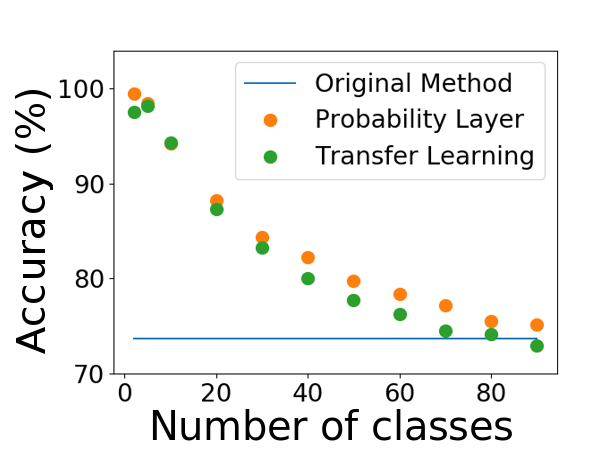
\includegraphics[width=\textwidth]{PLvsRetrain.png}
        \caption{Performance on different number of classes}
        \label{fig:PLvsRetrain}
  \end{minipage}
  \hfill
  \begin{minipage}[b]{0.235\textwidth}
        \centering
        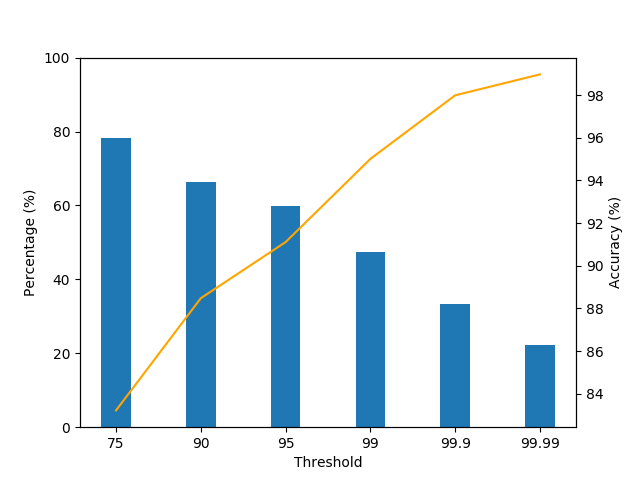
\includegraphics[width=\textwidth]{threshold.png}
        \caption{Threshold}
        \label{fig:threshold}
  \end{minipage}
\end{figure}

\begin{figure}
    \centering
    \begin{subfigure}[b]{0.235\textwidth}
        \centering
        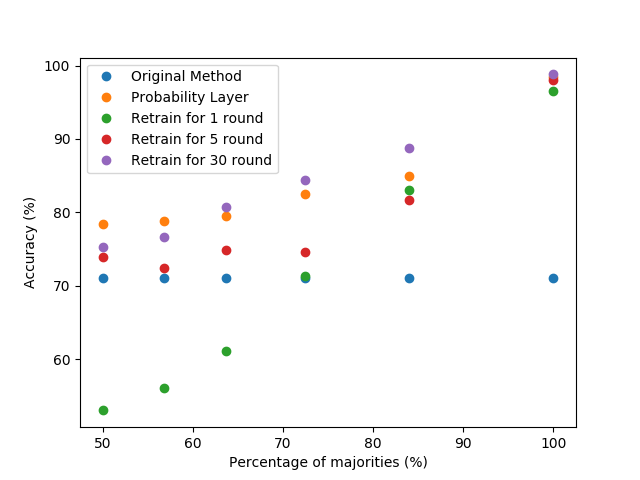
\includegraphics[width=\textwidth]{variousPercentage5.png}
        \caption{Five classes with various distribution}
        \label{fig:variousDistribution5}
    \end{subfigure}
    \begin{subfigure}[b]{0.235\textwidth}
        \centering
        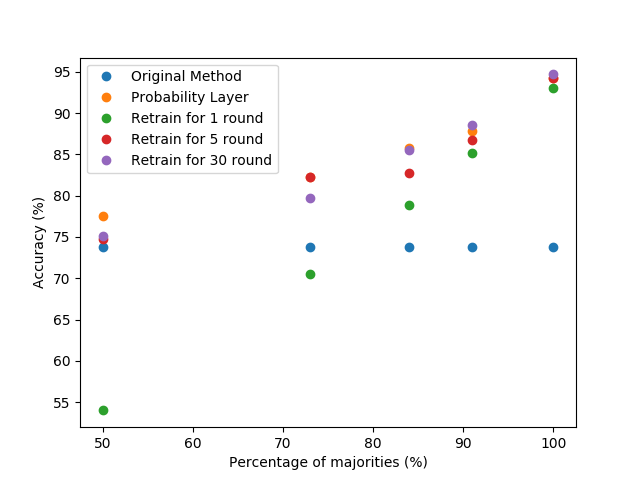
\includegraphics[width=\textwidth]{variousPercentage10.png}
        \caption{Ten classes with various distribution}
        \label{fig:variousDistribution10}
    \end{subfigure}

    \caption{Probability layer on denseNet}\label{fig:complex}
\end{figure}




\subsection{Results on specialized datasets with both majority and minority classes}
We evaluate the probability layer on the noisy environment, in which a few major classes occupies most of the images while a huge number of minority classes also appear. Figure \ref{fig:variousDistribution5} and Figure \ref{fig:variousDistribution10} shows the results when the numbers of majority classes are five and ten respectively. While the weight of majority classes increases from $50$\% to $100$\%, probability layer performs consistently better than the transfer learning for $5$ or $1$ epochs. Even if we finetune the model for $30$ rounds, probability layer still performs better when the weight of major classes is relatively small. When the weights increase further, the advantage of finetuning for $30$ rounds is at most $0.5$\%. Considering the intensive energy-consumption and time latency of retraining for $30$ rounds, this benefit of $0.5$\% advantage is not so significant, especially on devices which require the real-time response and has strict energy budget. We should also note that retraining for $1$ rounds would make the accuracy to be much lower than original model when the weight of major classes is less than 75\%. This phenonmenon cannot be contributed to the selection of hyper-parameters, i.e., learning rate and initialization methods, since virous learning rate has been tested manually and no significant difference is found. Since we need to choose a method before we start in automatically using environment information, we can conclude that probability layer is the most suitable method.




\begin{table}
    \caption{Perforation as a general pruning methods}
    \label{tab:generalPrune}

    \centering
    \begin{tabular}{ c|c|cc } 
     \hline
     Network & Acc. (\%) & Para. (M) & Com. (M) \\ 
     \hline
     AlexNet \cite{ahmed2016network, NIPS2012_4824} & 56.12 & 57.26 & 302.10 \\
     SqueezeNet \cite{iandola2016squeezenet} & 56.73 & 0.78 & 730.10 \\
     \hline
     Dense-40 \cite{huang2017densely} & 72.45 & 1.12 & 264.85 \\
     Dense-13 \cite{huang2017densely}& 58.89 & 0.09 & 21.88 \\
     \hline
     DenseP A (Ours)& 71.26 & 1.12 & 139.49 \\
     DenseP B (Ours)& 61.61 & 0.10 & 24.90 \\
     \hline
    \end{tabular}
\end{table}

\begin{table}
    \caption{Class-specific pruning}
    \label{tab:csPruning}

    \centering
    \begin{tabular}{ c|c|cc } 
     \hline
     Network & Acc. (\%) & Parameters & Computation \\ 
     \hline
     2 classes A & 72.45 & $P_A$ & $C_A$ \\
     2 classes B & B & $P_A$ & $P_B$ \\
     2 classes B & 72.45 & $P_B$ & $C_B$ \\
     \hline
     5 classes C & 72.45 & $P_A$ & $C_A$ \\
     5 classes D & B & $P_A$ & $P_B$ \\
     5 classes D & 72.45 & $P_B$ & $C_B$ \\
     \hline
     Original Model & 72.45 & P & C \\
     \hline
    \end{tabular}
\end{table}





\begin{table}
    \centering
    \begin{tabular}{c|ccc|ccc}
    \hline
    \multirow{2}{*}{Segments} & \multicolumn{3}{c|}{disabled} &  \multicolumn{3}{c}{enabled}\\
        & Acc & Para & Comp & Acc & Para & Comp    \\
    \hline
    (random)      & 72.45 & A & M & 72.45 & A & M \\
    \hline
    (n=5,p=.9)      & \multirow{2}{*}{A} & \multirow{2}{*}{L} & \multirow{2}{*}{A} & \multirow{2}{*}{L} \\
    +(random) & & & & \\
    \hline
    (n=5,p=.9)      & \multirow{2}{*}{A} & \multirow{2}{*}{L} & \multirow{2}{*}{A} & \multirow{2}{*}{L} \\
    +(random) & & & & \\
    
    \hline
    (n=15,p=.9)      & \multirow{2}{*}{A} & \multirow{2}{*}{L} & \multirow{2}{*}{A} & \multirow{2}{*}{L} \\
    +(n=10,.8) & & & & \\
    \hline

    
    \end{tabular}
    \caption{Results on synthesized datasets}
    \label{tab:synthe}
\end{table}




\subsection{Perforation}
Table \ref{tab:generalPrune} shows the effect of perforation as a general pruning methods.

Table \ref{tab:csPruning} shows the effect of perforation on class-specific pruning.

\subsection{Overall: Synthetic experiments}


\subsection{Overall: Video experiments}


\newpage
\clearpage
\section{Related Work} \label{relatedWork}
SECS is a real-time deep stream processing system utilizing runtime class skew efficiently and conducting class specific pruning automatically.

\paragraph{Class skew}
Using class skew is an emerging method for both increasing accuracy and decreasing resource consumption \cite{han2016mcdnn, kang2017noscope, shen2016fast}. Our paper is distinguished from existing papers from two main points. First, we bring up probability layer to efficient adapt the model with no overhead, while existing papers relies on transfer learning to finetune the model towards the class skew during runtime. Specifically, our probability layer introduce no overhead into the runtime model adaption, which fits more for the resource-limited nature on mobile platforms. Secondly, we identify the class skew dichotomy and bring up two modes, interpretation and compilation, to optimize model differently according to whether a class skew is hot or not. Third, we propose class-specific pruning and bring up perforation to efficiently select the smallest model according to whether the targetting class groups is hard to classify or not.


% Talk about transfer learning
\paragraph{Transfer learning}
Transfer learning has shown benefit in domain adaption and currently is the dominant method, if not the only one, for domain adaption. To solve the problem that the testing dataset is small, we use transfer learning \cite{oquab2014learning}. To use unsupervised dataset \cite{doersch2015unsupervised, noroozi2016unsupervised}, we use transfer learning. Assume we have a large model handling $1000$ classes and in an environment where only $10$ classes appearing, we still use transfer learning \cite{han2016mcdnn, shen2016fast}. Transfer learning has become the only method off the top of the head when we consider the change in classes. Although transfer learning shows various benefit, it also has intrinsic shortage residing in the process of training a CNN model. First, it is hard to decide how many layers we should freeze. Published papers \cite{yosinski2014transferable} reported that freezing fewer layers leads to better performance on different domains and freezing more layers lead to a better performance on similar domains since the co-adapted interactions between layers will be kept. However, it is still hard to decide whether two domains are similar enough and the exact effect of freezing a various number of layers. Second, transfer learning is hard to be conducted unless different settings has been tried. When choosing epoch numbers, it is hard to predict whether the model will converge or collapse after a pre-chosen number of epochs. The choice of learning rate also depends on both model and dataset. The choice of hyper-parameter needs expertise in finetuning, which is lacked by the automatical product. Third, the long latency and energy consumption of training a model obstacle the transfer learning on energy-efficient devices, especially in an environment that class number and distributions keep changing. Our approach, probability layer, can avoid finetuneing at all while adapting to the new dataset, thus all the inconvenience related to finetuneing is avoided naturally.

\paragraph{Model architecture selection.}
To generate a cascade of models with different resource consumption and performance, existing papers utilize hand-selected architectures, which is not a automatical procedure and only a small number of hyperparameters can be tested. Specifically, NoScope \cite{kang2017noscope} only performs model search by varying the number of convolutional layers (2 or 4), number of convolution units in the base layer (32 or 64), and number of neurons in the fully connected layer (32, 64, 128, or 256). MCDNN \cite{han2016mcdnn} chooses between reduce number of nodes in fully connected layers, decrease number of kernels, and eliminate convolutional layers entirely. FastVideo \cite{shen2016fast} also manually removes layers, decreases kernel sizes, increases kernel strides, and reduces the size of fully-connected layers, to generate a cascade of models with the tradeoff between accuracy and resource consumption. All these manually selected architectures requires human interfere. We observe that the difficulty comes from getting the exact accuracy of each architecture and loose the target to be collecting the relative performance of a sequence of architectures. Further, we bring up perforation to automatically se-lect hyper-parameters according to the targetting classeswithout any finetuning during the selection process.


\paragraph{Model compression}
Various model compression methods has been brought up, including matrix factorization \cite{jaderberg2014speeding, kim2015compression, romero2014fitnets, xue2014singular}, matrix pruning \cite{chen2015compressing, han2015learning}, and distillation \cite{hinton2015distilling, ba2014deep, dauphin2013big, chen2017learning, lopez2015unifying, kim2015compression,bucilu2006model}. Matrix factorization utilizes the multiplication of two low rank matrices to replace a single high rank matrix. In matrix pruning, the matrix is transformed into sparse matrix by pruning small digits to be zero. Distillation is another pruning methods, in which a complex model can teach a smaller model to get a better performance and the smaller model can replace the complex model for the reduction in resource consumption. After we conduct class-specific pruning, all these methods could be utilized to further reduce resource consumption, which will be covered in the future work.

\paragraph{Early stop}
Early stop \cite{teerapittayanon2016branchynet, panda2016conditional} is an architecture with branches and will stop calculating once a branch is enough confident that an image has been classified correctly. Early stop contains various architectures to achieve energy efficiency through reducing unnecessary computation. This is orthogonal to runtime specialization and could be included into the model bank.

\section{Conclusion and Future Work} \label{conclusion}
We have presented SECS, a real-time deep stream processing system. We identified an environment class skew, that is easily available and can both increase accuracy and decrease resource consumption. Probability layer is brought up to efficiently utilize the class skew. We further identified the class skew dichotomy. To conduct class-specific pruning for hot class skews, we propose perforation, which can bring extra benefit based on whether not a group of classes is easy to classify.


\newpage
\clearpage



\bibliographystyle{plain}
\bibliography{references}


\end{document}


